% Options for packages loaded elsewhere
\PassOptionsToPackage{unicode}{hyperref}
\PassOptionsToPackage{hyphens}{url}
%
\documentclass[
]{article}
\usepackage{amsmath,amssymb}
\usepackage{lmodern}
\usepackage{iftex}
\ifPDFTeX
  \usepackage[T1]{fontenc}
  \usepackage[utf8]{inputenc}
  \usepackage{textcomp} % provide euro and other symbols
\else % if luatex or xetex
  \usepackage{unicode-math}
  \defaultfontfeatures{Scale=MatchLowercase}
  \defaultfontfeatures[\rmfamily]{Ligatures=TeX,Scale=1}
\fi
% Use upquote if available, for straight quotes in verbatim environments
\IfFileExists{upquote.sty}{\usepackage{upquote}}{}
\IfFileExists{microtype.sty}{% use microtype if available
  \usepackage[]{microtype}
  \UseMicrotypeSet[protrusion]{basicmath} % disable protrusion for tt fonts
}{}
\makeatletter
\@ifundefined{KOMAClassName}{% if non-KOMA class
  \IfFileExists{parskip.sty}{%
    \usepackage{parskip}
  }{% else
    \setlength{\parindent}{0pt}
    \setlength{\parskip}{6pt plus 2pt minus 1pt}}
}{% if KOMA class
  \KOMAoptions{parskip=half}}
\makeatother
\usepackage{xcolor}
\IfFileExists{xurl.sty}{\usepackage{xurl}}{} % add URL line breaks if available
\IfFileExists{bookmark.sty}{\usepackage{bookmark}}{\usepackage{hyperref}}
\hypersetup{
  pdftitle={Variables estadísticas bidimensionales},
  hidelinks,
  pdfcreator={LaTeX via pandoc}}
\urlstyle{same} % disable monospaced font for URLs
\usepackage[margin=3cm]{geometry}
\usepackage{longtable,booktabs,array}
\usepackage{calc} % for calculating minipage widths
% Correct order of tables after \paragraph or \subparagraph
\usepackage{etoolbox}
\makeatletter
\patchcmd\longtable{\par}{\if@noskipsec\mbox{}\fi\par}{}{}
\makeatother
% Allow footnotes in longtable head/foot
\IfFileExists{footnotehyper.sty}{\usepackage{footnotehyper}}{\usepackage{footnote}}
\makesavenoteenv{longtable}
\usepackage{graphicx}
\makeatletter
\def\maxwidth{\ifdim\Gin@nat@width>\linewidth\linewidth\else\Gin@nat@width\fi}
\def\maxheight{\ifdim\Gin@nat@height>\textheight\textheight\else\Gin@nat@height\fi}
\makeatother
% Scale images if necessary, so that they will not overflow the page
% margins by default, and it is still possible to overwrite the defaults
% using explicit options in \includegraphics[width, height, ...]{}
\setkeys{Gin}{width=\maxwidth,height=\maxheight,keepaspectratio}
% Set default figure placement to htbp
\makeatletter
\def\fps@figure{htbp}
\makeatother
\setlength{\emergencystretch}{3em} % prevent overfull lines
\providecommand{\tightlist}{%
  \setlength{\itemsep}{0pt}\setlength{\parskip}{0pt}}
\setcounter{secnumdepth}{5}
\ifLuaTeX
  \usepackage{selnolig}  % disable illegal ligatures
\fi



\title{Variables estadísticas bidimensionales}
\author{}
\date{}

\hypersetup{
colorlinks=true,
    urlcolor=PineGreen,
    citecolor=PineGreen,
}
\usepackage{fancyhdr}
\usepackage{caption}
\pagestyle{empty}
\pagestyle{fancy}

\fancyhead[LE,RO]{Variables estadísticas bidimensionales}
\fancyhead[LO,RE]{}
\fancyfoot[LE,RO]{\thepage}
\fancyfoot[C]{}

\renewcommand{\familydefault}{\sfdefault}

\begin{document}




\maketitle

En ocasiones los datos se presentan en pares \((x,y)\). Es decir que al
recoger los datos no solo tenemos una variable, sino dos y hay una
correspondencia entre los valores de una y los de la otra.

Pensemos en el siguente ejemplo:

\hypertarget{ejemplo}{%
\subsubsection{Ejemplo}\label{ejemplo}}

Una empresa observa que parece haber una relación fuerte entre las
ventas en enero y las ventas en febrero. Para ello se recogen los datos
de 9 años y se anotan en una tabla las ventas de enero y febrero de cada
año en miles de euros.

\begin{longtable}[]{@{}ll@{}}
\toprule
ventas enero & ventas febrero\tabularnewline
\midrule
\endhead
142.74 & 69.06\tabularnewline
146.58 & 70.62\tabularnewline
149.01 & 72.03\tabularnewline
151.72 & 73.48\tabularnewline
154.12 & 74.89\tabularnewline
158.23 & 76.48\tabularnewline
160.19 & 77.85\tabularnewline
165.46 & 79.54\tabularnewline
168.82 & 81.05\tabularnewline
\bottomrule
\end{longtable}

Para analizar estos datos, podríamos trabajar con cada variable por
separado (calculando medias, varianzas, haciendo gráficas\ldots{}), pero
se perdería la relación entre ambas. Siguendo este procedimiento sería
dificil observar por ejemplo como a mayores ventas en enero corresponden
mayores ventas en febrero.

Para ello trabajamos con las dos variables juntas, a través de la
\textbf{Covarianza} y el \textbf{coeficiente de correlación de pearson}.
Mediante ellos intentaremos capturar la relación de dependencia entre
ambas variables, particularmente la \emph{dependencia lineal,}, que
ocurre cuando una de las variables puede ser aproximadas a partir de la
otra mediante una recta.

\hypertarget{covarianza}{%
\section{Covarianza}\label{covarianza}}

La \textbf{covarianza} es un valor que indica el grado de variación
conjunta de dos variables aleatorias respecto a sus medias. Es el dato
básico para determinar si existe una dependencia entre ambas variables y
además es el dato necesario para estimar otros parámetros básicos, como
el coeficiente de correlación lineal.

Supongamos que tenemos unos datos
\[(x_1, y_1), (x_2, y_2), (x_3,y_3), \ldots (x_N,y_N)\]

La covarianza se denota por \(S_{xy}\) y se define como

\[ S_{xy} = \frac{1}{N}\sum^N_{i=1}(x_i - \overline{x})(y_i - \overline{y}) \]
\[ =\frac{1}{N}((x_1- \overline x)(y_1 - \overline y)+ (x_2- \overline x)(y_2 - \overline y)+ \ldots +(x_N- \overline x)(y_N - \overline y))\]

donde \(\overline x\) denota la media de la primera variable (\(x\)), e
\(\overline y\) denota la media de la segunda (\(y\))

\hypertarget{ejemplo-1}{%
\subsection{Ejemplo}\label{ejemplo-1}}

Para entender cómo calcularlo, usaremos el ejemplo anterior. Primero
calculamos la media de ambas variables. En este caso como todos los
datos son distintos no hay frecuencias así que para calcular las medias
basta sumar y dividir entre el número de datos.

Obtenemos \(\overline x \cong155.207\), \(\overline y \cong77.337\).
Añadimos una columna calculando las multiplicaciones
\((x_i - \overline{x})(y_i - \overline{y})\)

\begin{longtable}[]{@{}lll@{}}
\toprule
\(x_i\) & \(y_i\) &
\((x_i - \overline{x})(y_i - \overline{y})\)\tabularnewline
\midrule
\endhead
142.74 & 69.06 & 80.389\tabularnewline
146.58 & 70.62 & 21.981\tabularnewline
149.01 & 72.03 & 16.658\tabularnewline
151.72 & 73.48 & 4.142\tabularnewline
154.12 & 74.89 & -1.916\tabularnewline
158.23 & 76.48 & -1.564\tabularnewline
160.19 & 77.85 & 2.502\tabularnewline
165.46 & 79.54 & 27.908\tabularnewline
168.82 & 81.05 & 114.372\tabularnewline
\bottomrule
\end{longtable}

y para calcular la covarianza basta sumar esta tercera columna y dividir
entre el número de datos

\[S_{xy} \cong 264.474/9 \cong 29.386\]

\hypertarget{el-gruxe1fico-nubes-de-puntos}{%
\subsection{El gráfico nubes de
puntos}\label{el-gruxe1fico-nubes-de-puntos}}

Una manera de visualizar la relación o dependencia entre las dos
variables es dibujar cada punto \((x_i, y_i)\) en el plano.

En el ejemplo anterior, el gráfico sería el siguente.

\begin{figure}
\centering
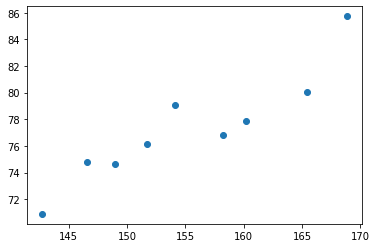
\includegraphics[width=3.64583in,height=\textheight]{cloud.png}
\caption{nube de puntos}
\end{figure}

\hypertarget{coeficiente-de-correlaciuxf3n-de-pearson}{%
\section{Coeficiente de correlación de
Pearson}\label{coeficiente-de-correlaciuxf3n-de-pearson}}

El coeficiente de \textbf{correlación de Pearson} es una medida de
dependencia lineal entre dos variables estadísticas cuantitativas. A
diferencia de la covarianza, la correlación de Pearson es independiente
de la escala de medida de las variables.

Se define como

\[\rho_{XY} = \frac{S_{xy}}{S_X S_Y}\]

donde \(S_{xy}\) de nota la covarianza, \(S_X\) denota la desviación
típica de la primera variable y \(S_Y\) la desviación típica de la
segunda.

en el ejemplo anterior, si calculamos además la desviación típica de
\(X\) e \(Y\) obtenemos

\[S_x \cong 8.205\] \[S_y \cong 3.920\]

luego

\[\rho_{XY}\cong\frac{29.386}{8.205 \cdot 3.920} \cong 0.913\]

Deducimos de aquí que dado que el coeficiente de correlación de Pearson
es cercano a 1 existe una dependencia lineal directa entre las ventas de
enero y febrero

\hypertarget{interpretaciuxf3n-del-coeficiente-de-correlaciuxf3n-de-pearson}{%
\subsection{Interpretación del coeficiente de correlación de
Pearson}\label{interpretaciuxf3n-del-coeficiente-de-correlaciuxf3n-de-pearson}}

\begin{itemize}
\item
  Si \(\rho_{XY}>{0}\) hay dependencia lineal directa (positiva), es
  decir, a grandes valores de \(X\) corresponden grandes valores de
  \(Y\).

  \begin{figure}
  \centering
  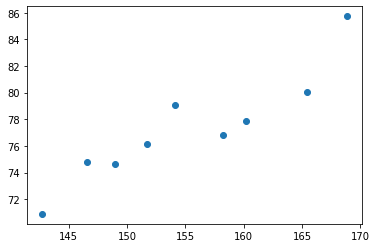
\includegraphics[width=2.60417in,height=\textheight]{cloud.png}
  \caption{nube de puntos correlación positiva}
  \end{figure}
\item
  Si \(\rho_{XY} ={0}\) se interpreta como la no existencia de una
  relación lineal entre las dos variables.

  \begin{figure}
  \centering
  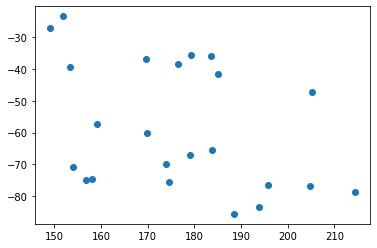
\includegraphics[width=2.60417in,height=\textheight]{cloud_cero.png}
  \caption{nube de puntos correlación 0}
  \end{figure}
\item
  Si \(\rho_{XY}<{0}\) hay dependencia lineal inversa o negativa, es
  decir, a grandes valores de \(X\) corresponden pequeños valores de
  \(Y\).

  \begin{figure}
  \centering
  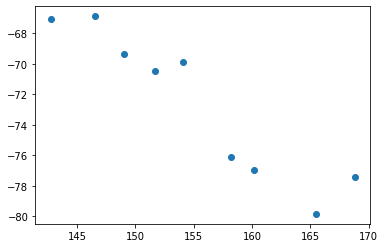
\includegraphics[width=2.60417in,height=\textheight]{cloud_menos.png}
  \caption{nube de puntos correlación negativa}
  \end{figure}
\end{itemize}

\hypertarget{ejercicios}{%
\section{Ejercicios}\label{ejercicios}}

\begin{enumerate}
\def\labelenumi{\arabic{enumi}.}
\item
  Los siguientes datos corresponden a los porcentajes de mortalidad
  obtenidos a dosis crecientes de un insecticida. Los resultados fueron
  los siguientes:

  \begin{longtable}[]{@{}ll@{}}
  \toprule
  Dosis & Mortalidad\tabularnewline
  \midrule
  \endhead
  0 & 5\tabularnewline
  1 & 7\tabularnewline
  5 & 10\tabularnewline
  10 & 16\tabularnewline
  15 & 17\tabularnewline
  20 & 25\tabularnewline
  25 & 26\tabularnewline
  30 & 30\tabularnewline
  \bottomrule
  \end{longtable}

  Calcula la covarianza y el coeficiente de correlación de Pearson e
  interprétalo
\end{enumerate}

\end{document}